%! TEX program = pdflatex
%% Mauricio Caceres Bravo <mauricio.caceres.bravo@gmail.com>

%----------------------------------------------------------------------
\documentclass{article}

\usepackage[summary]{brownpreamble}
\usepackage{etoc}
\setcounter{tocdepth}{3}

\renewcommand{\subsectionmark}[1]{\markboth{#1}{}}
\renewcommand\sectiontype{Lecture \thesection:\ }
\lhead{\color{light-gray} \itshape Math Camp Aug 16, 2022 -- Lecture \thesection}
\rhead{\color{light-gray} \itshape \thesubsection. \leftmark}
\setcounter{section}{1}
% \renewcommand\SetHideLevel{1pt}
\titleformat{\section}[display]{\sectionstyle}{\sectiontype #1}{0pt}{\vspace{15pt}}

% \let\oldquote\quote
% \let\endoldquote\endquote
% \RenewDocumentEnvironment{quote}{om}
%   {\oldquote}
%   {\par\nobreak\smallskip
%    \hfill(#2\IfValueT{#1}{~---~#1})\endoldquote
%    \addvspace{\bigskipamount}}

%----------------------------------------------------------------------
\begin{document}
\displayoptions

% ---------------------------------------------------------------------
\section{Sequences, Continuity}
\label{sec:sequences_continuity}

\localtableofcontents

% ---------------------------------------------------------------------
\subsection{Sequences}
\label{sub:sequences}

A sequence is a collection of elements of a set indexed by the natural numbers. We will not be terribly precise with notation,\footnote{Formally, a sequence is an element of the infinite Cartesian product of $\mathbb{R}^N \times \ldots \times \mathbb{R}^N$. While tempting to define a sequence as a countable or finite subset of $\mathbb{R}^N$, sets have no notion of order; further, sequences can have repeated elements.} and denote sequences with elements in $S$ as $(x_m) \in S$.
\begin{definition}
  Let $(x_m) \in S$ be a sequence:
  \begin{enumerate}[a)]
    \item $(x_m)$ is \keyword{increasing} if $\forall m$ we have $x_m \le x_{m + 1}$; it is \textit{strictly} increasing if $x_m < x_{m + 1}$.
    \item $(x_m)$ is \keyword{decreasing} if $\forall m$ we have $x_m \ge x_{m + 1}$; it is \textit{strictly} decreasing if $x_m > x_{m + 1}$.
    \item $(x_m)$ is (strictly) \keyword{monotonic} if it is (strictly) increasing or decreasing .
    \item $(y_k)$ is a \keyword{subsequence} of $(x_m)$ if $\exists$ some strictly increasing sequence $(n_k) \in \mathbb{N}$ s.t. $y_k = x_{m_k}$.
    \item $(x_m)$ is bounded above, below, or bounded if $\set{x_m}_{m \in \mathbb{N}}$ is bounded above, below, or bounded (resp).
    \item $(x_m) \to +\infty$ if $\forall N > 0 ~~ \exists M$ s.t. $m \ge M \implies x_m \ge M$.  $(x_m) \to -\infty$ if $\forall N < 0 ~~ \exists M$ s.t. $m \ge M \implies x_m \le M$. If either property holds, we say the sequence $(x_m)$ \keyword{diverges}.
  \end{enumerate}
\end{definition}

\subsubsection{Convergence}
\label{ssub:convergence}

\begin{definition}[convergence]\label{def:lecture2_convergence}
  A sequence $x_m$ \keyword{converges} to $x$ if $\forall \varepsilon > 0 ~~ \exists M \in \mathbb{N}$ s.t. $d(x_m, x) < \varepsilon$ whenever $m \ge M$. We denote this as $x_m \to x$ or $\lim_{m \to \infty} x_m = x$.
\end{definition}

We can visualize this idea in the figure below: $x_m$ is eventually contained within any $\varepsilon$-ball if $x$.\footnote{Recall $\varepsilon$-ball is the equivalent of a neighborhood in Euclidean space, even through here in two dimensions it's technically a $\varepsilon$-circle.} \begin{figure}[H]
  \centering
  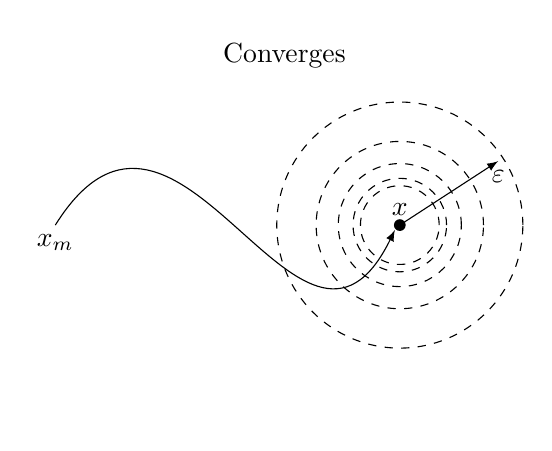
\begin{tikzpicture}[scale=1.25]
    \node [above, align=flush center] at (-1.125, 1.5) {
        Converges
    };
    \node[above] at (0, 0) {$x$};
    \node at (0, 0) [circle, fill, inner sep = 1.5pt] {};
    \draw [dashed] (0, 0) circle [radius=0.4];
    \draw [dashed] (0, 0) circle [radius=0.475];
    \draw [dashed] (0, 0) circle [radius=0.625];
    \draw [dashed] (0, 0) circle [radius=0.850];
    \draw [dashed] (0, 0) circle [radius=1.250];

    \draw [->, >=latex] (0, 0) -- (1, 0.65)
      node[below] at (1, 0.65) {$\varepsilon$};
    \draw [->, >=latex]
      (-3.5, 0)
        ..
        controls
          (-2.25, 2) and
          (-1, -2)
        ..
      (-0.05, -0.05)
    node[below] at (-3.5, 0) {$x_m$};
  \end{tikzpicture}
  \hspace{1.5cm}
  \begin{tikzpicture}[scale=1.25]
    \node [above, align=flush center] at (-1.225, 1.5) {
        Does not converge
    };
    \node[above] at (0, 0) {$x$};
    \node at (0, 0) [circle, fill, inner sep = 1.5pt] {};

    \draw [dashed] (0, 0) circle [radius=0.850];
    \node at (1.15, 0) [circle, fill, inner sep = 1.5pt] {};

    \draw [->, >=latex] (0, 0) -- (0.7, 0.45)
      node[below] at (0.65, 0.4) {$\varepsilon$};
    \draw [->, >=latex]
      (-3.5, 0)
        ..
        controls
          (-2.25, 2) and
          (-1, -2)
        ..
      (1.1, -0.05)
    node[below] at (-3.5, 0) {$x_m$};
  \end{tikzpicture}
\end{figure}
\vspace{-24pt}

\begin{claim}
  A sequence converges to at most one limit.
\end{claim}

\begin{proof}
  This is a consequence of the fact $d(x, y) \iff x = y$. Suppose $x_m \to x$ and $x_m \to y$. If $x \ne y$, then $d(x, y) > 0$. Take $\varepsilon = d(x, y)$; we know by the definition of convergence that there is some $M_x, M_y$ s.t. for $m \ge M = \max\Fset{M_x, M_y}$ we get
  \[
    d(x_m, x) < \varepsilon / 2
    \quad
    \text{and}
    \quad
    d(x_m, y) < \varepsilon / 2
  \]

  Now the triangle inequality gives
  \[
    \varepsilon
    =
    d(x, y)
    \le
    d(x_m, x) + d(x_m, y)
    <
    \varepsilon / 2
    +
    \varepsilon / 2
    =
    \varepsilon
    =
    d(x, y)
  \]

  contradiction ($\varepsilon < \varepsilon$). Hence $d(x, y) = 0$, or $x = y$.
\end{proof}

\begin{theorem}\label{thm:lecture2_closed_sequential}
  $S$ is closed $\iff$ for any $(x_m) \in S$ s.t. $x_m \to x$ for some $x \in \mathbb{R}^N$, we have that $x \in S$.
\end{theorem}

This is an equivalent definition of closedness: A set that ``contains all its limits.''
\begin{proof}
  See \Cref{ssub:sets_and_sequences_visualization_}.
  % First we show $S$ closed $\implies$ $S$ has all its limits. $S$ is closed in a metric space $X$ if $X \setminus S$ is open. Suppose $\exists (x_m) \in S^\infty$ s.t. $x_m \to x$ and $x \in X \setminus S$. That means that $\exists \varepsilon > 0$ s.t.  $B_{\varepsilon}(x) \subset X \setminus S$.  But by definition of convergence, $\exists M$ s.t. $m \ge M$ gives $x_m \in B_{\varepsilon}(x) \subseteq X \setminus S$, so $x_m \notin S$, a contradiction.
  %
  % Now we show that $S$ closed $\impliedby$ $S$ has all its limits. We proceed by contrapositive: Suppose that $S$ is not closed, then we will show it does not have all its limits. $X \setminus S$ is not open, so for some $x \in X \ S$ we have that for \textit{every} $\varepsilon > 0$, $B_{\varepsilon}(x) \cap S \ne \varnothing$ (i.e. it is not contained in $X \setminus S$).
  %
  % Take $1/m = \varepsilon_m$ for each $m = 1, 2, 3, \ldots$; we know that $\exists x_m$ s.t. $x_m \in B_{\varepsilon_m}(x)$. Now take an arbitrary $\varepsilon > 0$; there is some $M \in \mathbb{N}$ s.t. $1 / M < \varepsilon$, so $m \ge M$ gives $x_m \in B_{\varepsilon}(x)$. Thus $x_m \to x$ but $(x_m) \in S^\infty$ and $x \notin S$, which is the contrapositive we wanted to show.
\end{proof}

\begin{theorem}
  Take any set $S \subseteq \mathbb{R}^N$; the following are equivalent:
  \begin{enumerate}[a)]
    \item $x \in \closure(S)$.
    \item $\forall \varepsilon > 0, B_{\varepsilon}(x) \cap S \ne \varnothing$.
    \item $\exists (x_m) \in S$ s.t. $x_m \to x$.
  \end{enumerate}
\end{theorem}

\begin{proof}
  We will cycle through the proofs. First we show $b \implies c$: Take any $x$ s.t. $b$ holds. Let $1/m = \varepsilon_m$ for each $m = 1, 2, 3, \ldots$; we know that $\exists x_m$ s.t. $x_m \in B_{\varepsilon_m}(x)$. Now take an arbitrary $\varepsilon > 0$; there is some $M \in \mathbb{N}$ s.t. $1 / M < \varepsilon$, so $m \ge M$ gives $x_m \in B_{\varepsilon}(x)$. Thus $x_m \to x$ with $(x_m) \in S$.

  Now we show that $c \implies a$. Note that for any closed $T$ s.t. $S \subseteq T$, we have that $(x_m) \in S \implies (x_m) \in T$. Since $T$ is closed and $x_m \to x$, $x \in T$ by \Cref{thm:lecture2_closed_sequential}. Since $S \subseteq \closure(S)$ and $\closure(S)$ is closed, both by definition, this proves that $c \implies a$.

  To finish, we show that $a \implies b$. Suppose that $x \in \closure(S)$ but for some $\varepsilon > 0$, $B_{\varepsilon}(x) \cap S = \varnothing$. This means that $B_{\varepsilon}(x) \subset \mathbb{R}^N \setminus S$. Since $B_{\varepsilon}(x)$ is open, $\closure(S) \setminus B_{\varepsilon}(x)$ is closed. Further, since $x \notin S$ (because $x \in B_{\varepsilon}(x)$ and $B_{\varepsilon}(x) \cap S = \varnothing$), we have that $S \subseteq \closure(S) \setminus B_{\varepsilon}(x)$.  Since $x \in \closure(S)$, this implies $\closure(S) \subset \closure(S) \setminus B_{\varepsilon}(x)$. At the same time, $\closure(S)$ is the intersection of \textit{every} closed set containing $S$, so $\closure(S) \setminus B_{\varepsilon}(x) \subseteq \closure(S)$. Thus $\closure(S) \subset \closure(S)$, a contradiction.
\end{proof}

\begin{definition}
  Let $(x_m)$ be any sequence. We define
  \[
    \limsup_{m \to \infty} = \lim_{m \to \infty} \left(\sup_{k \ge m} x_k\right)
  \]

  and
  \[
    \liminf_{m \to \infty} = \lim_{m \to \infty} \left(\inf_{k \ge m} x_k\right)
  \]
\end{definition}

The $\limsup$ and $\liminf$ do not require convergence. Take, for instance, $(x_m) = 0, 1, 0, 1 \ldots$. Clearly $\limsup = 1$ and $\liminf = 0$ but the limit does not exist.

\subsubsection{Sets and Sequences (Visualization)}
\label{ssub:sets_and_sequences_visualization_}

The mathy sequel to Dungeons \& Dragons. In this section we will try to visualize the proof of \Cref{thm:lecture2_closed_sequential}. This should give some intuition for why convergence is related to sets being closed beyond the formality of the theorem.
\begin{itemize}[label=$\bullet$]
  \item If a sequence $x_m$ converges to $x$, then it becomes arbitrarily close to a point. If for every $(x_m) \in A$ s.t. $x_m \to x$ we also have $x \in A$, that means that no sequence can ever ``escape '' outside of $A$:
    \begin{figure}[H]
      \centering
      \begin{tikzpicture}
        \begin{axis}[name=plot1
          %,title=
          ,width=12cm
          ,height=8cm
          ,ymin=0
          ,ymax=6
          ,xmin=0
          ,xmax=8
          ,domain=0:8
          %,ylabel=$y$
          %,xlabel=$x$
        ]
          \draw [fill=shadecolor] (axis cs:3, 3) circle [blue, radius=2] ;
          \addplot [only marks, mark=*] coordinates {(4.41, 4.41) (1.59, 1.59)};

          \node[left] at (axis cs:1.59, 1.59) {$x$};
          \node[above] at (axis cs:2.75, 1.75) {$x_m$};
          \node[right] at (axis cs:4.41, 4.41) {$x^\prime$};
          \node[above] at (axis cs:3.2, 4.2) {$x_m^\prime$};

          \draw [dashed, ->, >=latex]
            (axis cs:2.75, 1.75) to[bend left=25] (axis cs:1.75, 1.55) ;

          \draw [dashed, ->, >=latex]
            (axis cs:3.2, 4.2) to[bend right=25] (axis cs:4.3, 4.4) ;

          % \draw [fill=white, dashed, line width=0.75]
          %   (axis cs:4.41, 4.41) circle [blue, radius=0.25] ;
          % \node [above] at (axis cs:4.75, 4.75) {$B_{\varepsilon}(x) \cancel{\subseteq} B$};
        \end{axis}
      \end{tikzpicture}
    \end{figure}

    By contrapositive, if $A$ is not closed, its complement is not open, so $\exists y \in \mathbb{R}^N \setminus A$ that cannot be enclosed in an $\varepsilon$-ball inside of $\mathbb{R}^N \setminus A$. In other words, there is some $y$ s.t. for each $\varepsilon_m = 1/m$ we can find a corresponding $y_m \in A$. The resulting $(y_m) \in A$ converges to $y \notin A$.
    \begin{figure}[H]
      \centering
      \begin{tikzpicture}
        \begin{axis}[name=plot1
          %,title=
          ,width=12cm
          ,height=8cm
          ,ymin=0
          ,ymax=6
          ,xmin=0
          ,xmax=8
          ,domain=0:8
          %,ylabel=$y$
          %,xlabel=$x$
        ]
          \draw [fill=shadecolor] (axis cs:3, 3) circle [blue, radius=2] ;
          \addplot [only marks, mark=*] coordinates {(4.41, 4.41) };

          \draw [fill=white, dashed, line width=0.75] (axis cs:4.41, 4.41) circle [blue, radius=0.6];
          \draw [dashed, line width=0.75] (axis cs:4.41, 4.41) circle [blue, radius=0.4];
          \draw [dashed, line width=0.75] (axis cs:4.41, 4.41) circle [blue, radius=0.2];

          \node [above] at (axis cs:5.25, 5.15) {$B_{\sfrac{1}{m}}(y) \cap  A \ne \varnothing ~~ \forall m$};

          \draw [->, >=latex, line width=1pt]
            (axis cs:2.95, 4.15) to[bend left=25] (axis cs:4.3, 4.4) ;
          \node[below] at (axis cs:2.95, 4.15) {$y_m \to y, y \notin A$};
        \end{axis}
      \end{tikzpicture}
    \end{figure}

    In other words, if $A$ is not closed, we can find a sequence that ``escapes'' $A$, which by contrapositive proves that if every sequence in $A$ that converges does so to a point in $A$, the set is closed.

  \item On the other hand, if $A$ is closed and we have a sequence $(y_m) \in A$ s.t. $y_m \to y$ with $y \notin A$, then we have a sequence that ``escaped'' $A$. However, $A$ closed implies $X \setminus A$ is open, and $\exists B_{\varepsilon}(y) \subseteq \mathbb{R}^N \setminus A$. Since $y_m$ will get arbitrarily close to $y$, $\exists y_m \in B_{\varepsilon}(y) \subseteq X \setminus A$. Since $y_m \in A$ by premise, this is a contradiction.
    \begin{figure}[H]
      \centering
      \begin{tikzpicture}
        \begin{axis}[name=plot1
          %,title=
          ,width=12cm
          ,height=8cm
          ,ymin=0
          ,ymax=6
          ,xmin=0
          ,xmax=8
          ,domain=0:8
          %,ylabel=$y$
          %,xlabel=$x$
        ]
          \draw [fill=shadecolor] (axis cs:3, 3) circle [blue, radius=2] ;
          \addplot [only marks, mark=*] coordinates {(5.11, 4.41)};

          \draw [fill=white, dashed, line width=0.75] (axis cs:5.11, 4.41) circle [blue, radius=0.4];
          \node [above] at (axis cs:5.25, 5.15) {$B_{\varepsilon}(y) \cap  A = \varnothing$};

          \draw [->, >=latex, line width=1pt]
            (axis cs:3.25, 3.95) to[bend left=25] (axis cs:5, 4.4) ;
          \node[below, text width = 3.85cm] at (axis cs:3.05, 3.95) {$y_m \to y$ and $y \notin A \implies \exists y_m \notin A$, contradiction};
        \end{axis}
      \end{tikzpicture}
    \end{figure}
\end{itemize}

I think in general it's very useful to visualize proofs in $\mathbb{R}^2$ (making drawings, as above):
\begin{itemize}[label=$\bullet$]
  \item $\mathbb{R}$ is not enough: A ton of things will hold in one dimension that won't in general, and one-dimensional intuition can end up being misleading.

  \item $\mathbb{R}^3$ can be too much: I cannot draw 3D very easily and it is harder to visualie clearly (certainly $\mathbb{R}^N$ would be too many dimensions).

  \item $\mathbb{R}^2$ is a nice trade-off between rigor an intuition.  (I know we discuss properties in more general terms than in $\mathbb{R}^2$, but for intuition I think it's a great benchmark.)
\end{itemize}

% Godel: https://www.youtube.com/watch?v=O4ndIDcDSGc

\subsubsection{Properties of Convergent Sequences}
\label{ssub:properties_of_convergent_sequences}

\begin{theorem}
  Take any sequence $(x_m) \in \mathbb{R}^N$:
  \begin{enumerate}[a)]
    \item $x_m \to x \implies x_{m_k} \to x$ for all subsequences $(x_{m_k})$ of $(x_m)$.

    \item $x_m \to x \implies (x_m)$ is bounded. (Is the converse true? Can you prove your answer?\footnote{A counterexample is sufficient: $x_m = (-1)^m$ is bounded above by $1$ and below by $-1$ but does not converge.})

    \item If $x_m \le y_m \le z_m$ and $x_m, z_m \to x$ then $y_m \to x$.

    \item If $x_m \to 0$ and $(y_m)$ is bounded then $x_m \cdot y_m \to 0$.
  \end{enumerate}

  Let $x_m \to x$ and $y_m \to y$:
  \begin{enumerate}[a)]\setcounter{enumi}{4}
    \item $c \cdot x_m \to c \cdot x$ for any $c \in \mathbb{R}$.

    \item $x_m \pm y_m \to x \pm y$.

    \item $x_m \cdot y_m \to x \cdot y$.

    \item $x_m / y_m \to x / y$ if $y \ne 0$.
  \end{enumerate}
\end{theorem}

% \begin{proof}
%   TODO: Should I prove all of these?
% \end{proof}

\subsubsection{Bolzano-Weierstrass}
\label{ssub:bolzano_weierstrass}

\begin{theorem}\label{thm:lecture2_bounded_mono_converge}
  Let $(x_m) \in \mathbb{R}$. If $(x_m)$ is bounded and monotonic then $(x_m)$ converges.
\end{theorem}

\begin{theorem}[Nested Intervals Theorem]\label{thm:lecture2_nested_interval}
  Let $I_m = [a_m,  b_m]$ s.t. $I_{m + 1} \subset I_m$.
  \begin{enumerate}[a)]
    \item $\cap_{m \in \mathbb{N}} I_m \ne \varnothing$
    \item If $b_m - a_m \to 0$ then $\cap_{m \in \mathbb{N}}$ is  a singleton.
  \end{enumerate}
\end{theorem}

\begin{proof}
  If $I_{m + 1} \subseteq I_m$, then $I_{m} \subseteq I_1$ for all $m$. Hence
  \[
    a_1 \le a_m \le a_{m + 1} \le b_{m + 1} \le b_m \le b_1
  \]

  for all $m$. In other words, $a_m$ and $b_m$ are bounded and monotonic, so $a_m \to a$ and $b_m \to b$ for some $a, b$ by \Cref{thm:lecture2_bounded_mono_converge}. Further, since $a_m \le b_m$ for all $m$, we have that $a \le b$ (do you see why?\footnote{If $a > b$ then we will have that $a_m > b_m$ for some $m$. That is, pick $0 < \varepsilon < a - b$; we can then find $M_a, M_b$ s.t.
    \[
      a - \varepsilon / 2 < a_m < a + \varepsilon / 2
      \quad\quad
      b - \varepsilon / 2 < b_m < a + \varepsilon / 2
    \]

    whenever $m > \max\set{M_a, M_b}$. However, $\varepsilon < a - b$ gives
    \[
      b_m < b + \varepsilon / 2 < a - \varepsilon / 2 < a_m
    \]

    Since $b_m \ge a_m$ for all $m$ we have a contradiction.}) and $I_m \to [a, b] \ne \varnothing$. If $b_m - a_m \to 0$, that means $b - a = 0$ so the interval $[a, b]$ is just the singleton $a = b$.
\end{proof}

\begin{theorem}[Bolzano-Weierstrass]
  Every bounded sequence in $\mathbb{R}$ admits a convergent sub-sequence.
\end{theorem}

\begin{proof}
  This follows from the \nameref{thm:lecture2_nested_interval} above---the trick is to construct the nested intervals, which we can do for bounded sequences. If $(x_m)$ is bounded, first define
  \[
    I_1 = [L, U] = [a_1, b_1]
  \]

  the interval with enpoints equal to the lower and upper bounds of $x_m$. Let $x_{m_1}$ the first element of the sub-sequence be any term of $x_m \in I_1$. Now take
  \[
    I_1^- = \left[a_1, \dfrac{a_1 + b_1}{2}\right]
    \quad\quad
    I_1^+ = \left[\dfrac{a_1 + b_1}{2}, b_1\right]
  \]

  and let $I_2 = I_1^-$ if $\set{x_m: m \in \mathbb{N}} \cap I_1^+$ is non-finite and $I_2 = I_1^+$ otherwise. Let $a_2, b_2$ be the endpoints of $I_2$ and $x_{m_2}$ be any term of $x_m \in I_2$. We iterate this process: In general
  \[
    I_k^- = \left[a_k, \dfrac{a_k + b_k}{2}\right]
    \quad\quad
    I_k^+ = \left[\dfrac{a_k + b_k}{2}, b_k\right]
  \]

  and $I_{k + 1} = I_k^-$ if $\set{x_m: m \in \mathbb{N}} \cap I_k^+$ is non-finite and $I_{n + 1} = I_k^+$ otherwise, with $x_{m_k}$ any element of $x_m \in I_k$. (What if both halves have a finite intersection?\footnote{Note that for $k > 1$, it must always be that either $I_k^+$ or $I_k^-$ have a non-finite intersection with $\set{x_m: m \in \mathbb{N}}$, since we chose $I_k$ to have a non-finite intersection.  The only way both halves will have a finite intersection is if $I_1$ is finite to begin with. However, this means that some $M$, $x_n = x_m$ whenever $n, m > M$, which means we have a convergent sub-sequence $x_{m_k} = x_{M + 1}$ with $m_k = M + k$.}) We have that
  \[
    a_1 \le a_{k - 1} \le a_k \le x_{m_k} \le b_k \le b_{k - 1} \le b_1
  \]

  Furthermore, $b_n - a_n = \dfrac{b_1 - a_1}{2^{n - 1}} \to 0$. Hence we can apply the \nameref{thm:lecture2_nested_interval}: $a_n \to a$ and $b_n \to b$ with $a = b$ implies $x_{m_k} \to a = b$.
\end{proof}

\subsubsection{Cauchy Sequences}
\label{ssub:cauchy_sequences}

\begin{definition}
  A sequence is \keyword{Cauchy} if $\forall \varepsilon > 0 ~~\exists M$ s.t.
  \[
    m, n > M \implies d(x_m, x_n) < \varepsilon
  \]
\end{definition}

\begin{theorem}
  If $(x_m)$ converges, then it is Cauchy.
\end{theorem}

\begin{proof}
  Suppose $x_m \to x$; by the triangle inequality
  \[
    d(x_m, x_n) \le d(x_m, x) + d(x_n, x)
  \]

  Now take any $\varepsilon > 0$; for $\varepsilon / 2$ we have that for some $M$, $m, n > M$ gives
  \[
    d(x_m, x) < \dfrac{\varepsilon}{2}
    \quad\quad
    d(x_n, x) < \dfrac{\varepsilon}{2}
  \]

  Hence
  \[
    d(x_m, x_n) \le d(x_m, x) + d(x_n, x) < \dfrac{\varepsilon}{2} +  \dfrac{\varepsilon}{2} = \varepsilon
  \]

  which shows $(x_m)$ is Cauchy.
\end{proof}

While the converse of the theorem above is also true in $\mathbb{R}^N$, during your math course you will probably encounter the fact that in general metric spaces, Cauchy sequences needn't converge. (The reason is, again, this property of Euclidean space called ``completeness.'')
\begin{theorem}
  If $(x_m)$ is a Cauchy sequence in $\mathbb{R}$ then $(x_m)$ converges.
\end{theorem}

\begin{proof}
  I will show this in $\mathbb{R}$: Cauchy sequences are bounded (why?), which means that there exist some sub-sequence $x_{m_k}$ that converges to some $x$. We show that this is also the limit for the sequence $x_m$. By the triangle inequality,
  \[
    d(x_m, x) \le d(x_m, x_{m_k}) + d(x_{m_k}, x)
  \]

  Take any $\varepsilon > 0$, then for $\varepsilon / 2$ we can find $K$ s.t. $k > K$ gives
  \[
    d(x_{m_k}, x) < \varepsilon / 2
  \]

  because $x_{m_k} \to x$, and $M$ s.t. $n, m_k > M$ gives
  \[
    d(x_m, x_{m_k}) < \varepsilon / 2
  \]

  because $x_m$ is Cauchy. Take $k > K$ s.t. $m_k \ge M$. Then for $n > M$ we have
  \[
    d(x_m, x) \le d(x_m, x_{m_k}) + d(x_{m_k}, x) < \varepsilon / 2 + \varepsilon / 2 = \varepsilon
  \]

  which is what we wanted to show. This proof should generalize to $\mathbb{R}^N$ if you argue that along each coordinate, $(x_m)$ is bounded and then use that to find a candidate limit $x$. Then the identical argument goes through (note it used generic properties of the distance rather than anything specific to $\mathbb{R}$).
\end{proof}

\begin{remark}
  The sticking point about ``completeness'' being required has to do with the fact the candidate limit $x$ needn't be in the space (e.g. take some sequence in $\mathbb{Q}$ that ``converges'' to $\pi \notin \mathbb{Q}$).
\end{remark}

% ---------------------------------------------------------------------
\subsection{Continuous Functions}
\label{sub:continuous_functions}

The intuition for continuity is that ``you can draw the function without picking up your pencil.'' (What about asymptotes like $1/x$ at $0$?\footnote{The intuition should still hold because the function is not defined at $0$; with infinitely long paper you needn't pick up your pencil.}) More precisely, if two points in the domain are close, the corresponding points in the co-domain must also be close. Put another way, a small neighborhood in the domain maps to a small neighborhood in the co-comain. (Note that the converse is not true! Take $f(x) = x^2$; $f(-x) = f(x) = x^2$, so the points are close in the image---they are identical---but as $x$ gets large, $x, -x$ get farther apart.)
\begin{figure}[H]
  \centering
  \caption{Intuition for Continuity}
  \label{fig:intuition_for_continuity}
  \begin{tikzpicture}
    \begin{axis}[name=plot1
      ,title={Continuous}
      ,width=9cm
      ,height=7cm
      ,ymin=0
      ,ymax=6
      ,xmin=0
      ,xmax=6
      ,domain=0:6
      ,ylabel=$f(x)$
      ,xlabel=$x$
    ]
    \draw [-, xshift=6pt] plot [smooth, tension=1]
      coordinates {
        (1.0, 1.0)
        (1.5, 2.0)
        (2.0, 1.5)
        (2.5, 3.0)
        (3.0, 2.5)
        (3.5, 4.0)
        (4.0, 3.5)
        (4.5, 4.5)
      };
    \draw [-, dashed] (axis cs:3.200, 2.55) -- (axis cs:3.200, 0);
    \draw [-, dashed] (axis cs:3.400, 3.15) -- (axis cs:3.400, 0);
    \draw [->, >=latex] (axis cs:2.9, 4.25) -- (axis cs:3.200, 2.60);
    \draw [->, >=latex] (axis cs:2.9, 4.25) -- (axis cs:3.400, 3.20);
    \node[above] at (axis cs:2.9, 4.25) {also close};

    \draw [->, >=latex] (axis cs:4.5, 1.25) -- (axis cs:3.225, 0.15);
    \draw [->, >=latex] (axis cs:4.5, 1.25) -- (axis cs:3.425, 0.15);
    \node[above] at (axis cs:4.5, 1.25) {close};
    \end{axis}

    \begin{axis}[name=plot2
      ,title={Not Continuous}
      ,at={($(plot1.east) + (0.5cm, 0)$)}
      ,anchor=west
      ,width=9cm
      ,height=7cm
      ,ymin=0
      ,ymax=6
      ,xmin=0
      ,xmax=6
      ,domain=0:6
      ,ylabel=$f(x)$
      ,xlabel=$x$
    ]
    \draw [-, xshift=6pt] plot [smooth, tension=1]
      coordinates {
        (0.5, 2.5)
        (1.0, 3.0)
        (1.5, 2.5)
        (2.0, 3.0)
        (2.5, 2.5)
        (2.75, 2.75)
        % (3.0, 3.0)
        % (3.5, 2.5)
        % (4.0, 3.0)
        % (4.5, 2.5)
      };
    \draw [-, xshift=6pt] plot [smooth, tension=1]
      coordinates {
        % (1.0, 3.0)
        % (1.5, 2.5)
        % (2.0, 3.0)
        % (2.5, 2.5)
        (2.75, 4.75)
        (3.0, 5.0)
        (3.5, 4.5)
        (4.0, 5.0)
        (4.5, 4.5)
        (5.0, 5.0)
      };

    \addplot [only marks, mark=*] coordinates {(2.925, 4.75)};
    \addplot [only marks, mark=*, color=white] coordinates {(2.925, 2.75)};
    \addplot [only marks, mark=o] coordinates {(2.925, 2.75)};
    \draw [-, dashed] (axis cs:2.925, 4.75) -- (axis cs:2.925, 0);

    \draw [->, >=latex] (axis cs:1.9, 3.75) -- (axis cs:2.825, 4.75);
    \draw [->, >=latex] (axis cs:1.9, 3.75) -- (axis cs:2.825, 2.75);
    \node[left] at (axis cs:1.75, 3.75) {not close};

    \draw [-, dashed] (axis cs:3.200, 4.90) -- (axis cs:3.200, 0);
    \draw [-, dashed] (axis cs:2.650, 2.50) -- (axis cs:2.650, 0);
    \draw [->, >=latex] (axis cs:3.9, 2.25) -- (axis cs:3.25, 0.15);
    \draw [->, >=latex] (axis cs:3.9, 2.25) -- (axis cs:2.70, 0.15);
    \node[above] at (axis cs:3.9, 2.25) {close};
    \end{axis}
  \end{tikzpicture}
\end{figure}

\begin{definition}[continuity]\label{def:continuity_continuous}
  A function $f: X \to Y$ is \keyword{continuous} at $x \in X$ if for every $\varepsilon > 0$ there exist a $\delta > 0$ s.t.
  \[
    d(z, x) < \delta
    \implies
    d(f(z), f(x)) < \varepsilon
  \]

  Put another way, $z \in B_{\delta}(x) \implies f(z) \in B_{\varepsilon}(f(x))$, or
  \[
    f(B_{\delta}(x))
    \subseteq
    B_{\varepsilon}(f(x))
  \]

  If $f$ is continuous at every $x \in X$ we say it is continuous.
\end{definition}

\begin{proposition}
  Let $\varphi: \mathbb{R}^N \to \mathbb{R}$. If $\varphi$ is continuous then the sets $\Fset{x \in \mathbb{R}^N: \varphi(x) \ge \alpha}$ and $\Fset{x \in \mathbb{R}^N: \varphi(x)\le \alpha}$ are closed for all $\alpha \in \mathbb{R}$.
\end{proposition}

\begin{proof}
  Let $A = \Fset{x \in \mathbb{R}^N: \varphi(x) \ge \alpha}$ and $B = \mathbb{R}^N \setminus A$. If $B$ is open then $A$ is closed. Note
  \[
    B = \Fset{
      x \in \mathbb{R}^N: \varphi(x) < \alpha
    }
  \]

  Pick any $x \in B$ and let $0 < \varepsilon < \alpha - \varphi(x)$. Then since $\varphi$ is continuous we know there is some $\delta > 0$ s.t.
  \[
    z \in B_{\delta}(x)
    \implies
    \varphi(x) - \varepsilon
    <
    \varphi(z)
    <
    \varphi(x) + \varepsilon
    <
    \alpha
    \implies
    z \in B
  \]

  therefore $B$ is open (for any point $\exists \delta$-ball that is entirely in $B$). Thus $\mathbb{R}^N \setminus B = A$ is closed. The proof for the lower sets is analogous.
\end{proof}

\begin{theorem}
  Let $f: X \to Y$ and $g: f(X) \subseteq Y \to Z$ with $X, Y, Z \subseteq \mathbb{R}^N$. If $f, g$ are continuous then $(g \circ f): X \to Z$ is continuous.
\end{theorem}

\begin{theorem}
  Let $f: X \to \mathbb{R}$ and $g: X \to \mathbb{R}$ be continuous functions. Then
  \begin{enumerate}
    \item $h(x) = f(x) \pm g(x)$ are continuous functions.
    \item $h(x) = f(x) \cdot g(x)$ is continuous.
    \item $h(x) = f(x) / g(x)$ is continuous whenever $g(x) \ne 0$.
  \end{enumerate}
\end{theorem}

% ---------------------------------------------------------------------
\subsection{Sequential and Open Set Characterizations}
\label{sub:sequential_and_open_set_characterizations}

\begin{remark}
  Continuous functions don't map open sets to open sets! Consider $f(x) = x^2$. The image of $(-2, 2)$ is $[0, 2)$, which is not open.  Further, evern if all maps of closed sets are closed, the function might not be continuous. For example, Consider a function that is $0$ if $x < 0$ and $1$ if $x \ge 1$. This has a jump at $1$, but $f([a, b])$ is either $\Fset{0}, \Fset{1},$ or $\Fset{0, 1}$, which are closed.

  Last, if a function is continuous the inverse image need not be. Consider a function $f: [0, 1) \to \mathbb{R}^2$ that maps the line into a circle:
  \begin{figure}[H]
    \centering
    \begin{tikzpicture}[scale=1]
      % original interval
       \draw [-] (-4, 0) -- (-1, 0);
       \draw [-] (-2.5, 0.25) -- (-2.5, -0.25);
       \draw [-] (-3.9, 0.25) -- (-4.0, 0.25) -- (-4.0, -0.25) -- (-3.9, -0.25);
       \draw [-] (-1.075, 0.25) to[bend left=35] (-1.075, -0.25);

       \node[below] at (-4, -0.25) {$0$};
       \node[below] at (-2.5, -0.25) {$1/2$};
       \node[below] at (-1, -0.25) {$1$};

      % function
       \draw [->, >=latex] (-0.75, 0.5) to[bend left=35] (0.5, 0.5);
       \node[above] at (-0.125, 0.75) {$f$};

       \draw [-] (2, 0) circle [radius=1.5];
       \draw [-] (2, 1.75) to[bend left=35] (2, 1.25);
       \draw [-] (2.2, 1.75) -- (2.1, 1.75) -- (2.1, 1.25) -- (2.2, 1.25);

       \filldraw (1.75, 1.475) circle (1.5pt);
       \filldraw (2.25, 1.475) circle (1.5pt);
       \node[above] at (1.75, 1.475) {$a$};
       \node[above] at (2.35, 1.475) {$b$};

      % inverse
       \draw [->, >=latex] (3.75, 0.5) to[bend left=35] (5.0, 0.5);
       \node[above] at (4.625, 0.75) {$f^{-1}$};

       \draw [-] (5, 0) -- (8, 0);
       \draw [-] (6.5, 0.25) -- (6.5, -0.25);
       \draw [-] (5.1, 0.25) -- (5.0, 0.25) -- (5.0, -0.25) -- (5.1, -0.25);
       \draw [-] (7.925, 0.25) to[bend left=35] (7.925, -0.25);

       \filldraw (5.5, 0) circle (1.5pt);
       \filldraw (7.5, 0) circle (1.5pt);
       \node[below] at (5.5, -0.25) {$f^{-1}(b)$};
       \node[below] at (7.5, -0.25) {$f^{-1}(a)$};
    \end{tikzpicture}
  \end{figure}

  We can  see that $a, b$ are close in the image, but not in the inverse image.
\end{remark}

The remarks above all get to the same idea: Continuity states that points in the image are close if the points in the domain are close, not the converse. Hence we have the following characterization in terms of the \textit{inverse image} and \textit{converging sequences}.
\begin{theorem}\label{thm:lecture2_continuity_open_closed}
  The following are equivalent for any $f: \mathbb{R}^N \to \mathbb{R}^M$:
  \begin{enumerate}[a)]
    \item $f$ is continuous.

    \item If $O \subseteq \mathbb{R}^M$ is open, $f^{-1}(O)$ is open.

    \item If $S \subseteq \mathbb{R}^M$ is closed, $f^{-1}(S)$ is closed.

    \item For every $(x_m) \in \mathbb{R}^N$ s.t. $x_m \to x$ for some $x \in \mathbb{R}^N$, $f(x_m) \to f(x)$.
  \end{enumerate}
\end{theorem}

\begin{proof}
  See \Cref{ssub:sets_and_continuity_visualization_}.
  % First, we prove $1 \implies 2$. Take any open set $S \in \mathbb{R}^M$ and any element $x \in f^{-1}(S)$. Since $S$ is open, for any $f(x) \in S$ there is some $\varepsilon > 0$ s.t. $B_{\varepsilon}(f(x)) \subseteq S$. Since $f$ is continuous, $\exists \delta$ s.t. $f(B_{\delta}(x)) \subseteq B_{\varepsilon}(f(x)) = B_{\varepsilon}(s) \subseteq S$, meaning $B_{\delta}(x) \subseteq f^{-1}(S)$, so $f^{-1}(S)$ is open.\footnote{The only sticking point here might be that $f(A) \subseteq B$ implies $A \subseteq f^{-1}(B)$ for any $f$. Note that $a \in A \implies f(a) \in B$, meaning for each $a \in A$ there is some $b \in B$ s.t. $f(a) = b$; by definition that means $a \in f^{-1}(B)$.}
  %
  % Now $2 \implies 3$. Let $S$ be any closed set in $\mathbb{R}^M$ and consider $f^{-1}(S)$. We know $O = \mathbb{R}^M \setminus S$ is open, and by assumption $f^{-1}(O) = f^{-1}(\mathbb{R}^M \setminus S) = \mathbb{R}^N \setminus f^{-1}(S)$ is open, meaning $f^{-1}(S)$ is closed.\footnote{The only sticking point here might be that $f^{-1}(\mathbb{R}^M \setminus S) = \mathbb{R}^N \setminus f^{-1}(S)$. Note that if a point $x$ is in $f^{-1}(\mathbb{R}^M \setminus S)$ then by definition there is no $s \in S$ s.t. $f(x) = s$; hence $x \notin f^{-1}(S)$, or $x \in \mathbb{R}^N \setminus f^{-1}(S)$. Similarly, if a point is $x \in \mathbb{R}^N \setminus f^{-1}(S)$ that means that $f(x) \notin S$, or that for every $s \in S$, $f(x) \ne s$, so $x \in f^{-1}(\mathbb{R}^M \setminus S)$.}
  %
  % Now $3 \implies 2$.  Let $O$ be any open set in $\mathbb{R}^M$ and consider $f^{-1}(O)$. We know $S = \mathbb{R}^M \setminus O$ is closed, and by assumption $f^{-1}(S) = f^{-1}(\mathbb{R}^M \setminus O) = \mathbb{R}^N \setminus f^{-1}(O)$ is closed, meaning $f^{-1}(O)$ is open.
  %
  % Now $2 \implies 4$. Let $(x_m) \in \mathbb{R}^N$ s.t. $x_m \to x$ for some $x \in \mathbb{R}^N$. Take any $\varepsilon > 0$. By assumption $f^{-1}(B_{\varepsilon}(f(x)))$ is open and $x \in f^{-1}(B_{\varepsilon}(f(x)))$ because $f(x) \in B_{\varepsilon}(f(x))$. Hence $\exists \delta > 0$ s.t. $B_{\delta}(x) \subseteq f^{-1}(B_{\varepsilon}(f(x)))$. Since $x_m \to x$, $\exists M$ s.t. $m \ge M \implies x_m \in B_{\delta}(x)$. That is, for $m \ge M$ there is some $y \in B_{\varepsilon}(f(x))$, $f(x_m) = y$, or $f(x_m) \in B_{\varepsilon}(f(x))$.  By definition that means $f(x_m) \to f(x)$.
  %
  % To finish, $4 \implies 1$.  Suppose that $f$ is not continuous at some point $x \in \mathbb{R}^N$. So $\exists \varepsilon > 0$ s.t. $\forall \delta > 0$,
  %   \[
  %     z \in B_{\delta}(x)
  %     \quad
  %     \text{and}
  %     \quad
  %     f(z) \notin B_{\varepsilon}(f(x))
  %   \]
  %
  % For each $m$, pick $x_m \in B_{1/m}(x)$ s.t. $f(x_m) \notin B_{\varepsilon}(f(x))$. By definition, $x_m \to x$, and by assumption $f(x_m) \to f(x)$, which is a contradiction (for some $M$, $m \ge M \implies f(x_m) \in B_{\varepsilon}(f(x))$, contradiction).
\end{proof}

\subsubsection{Sets and Continuity (Visualization)}
\label{ssub:sets_and_continuity_visualization_}

We show \Cref{thm:lecture2_continuity_open_closed} using, again, drawings in $\mathbb{R}^2$.
\begin{proof}
  We cycle through the statements. If we show $a \implies b \implies c \implies d \implies a$ then we have shown they are equivalent.
  \begin{enumerate}[1.]
    \item $a \implies b$. First, it is a good idea to write down what you have and what you want to show:
      \begin{itemize}[label=$\bullet$]
        \item Continuity means that $\forall \varepsilon > 0 ~~ \exists \delta > 0$ s.t. $z \in B_{\delta}(x) \implies f(z) \in B_{\varepsilon}(f(x))$.
        \begin{figure}[H]
          \centering
          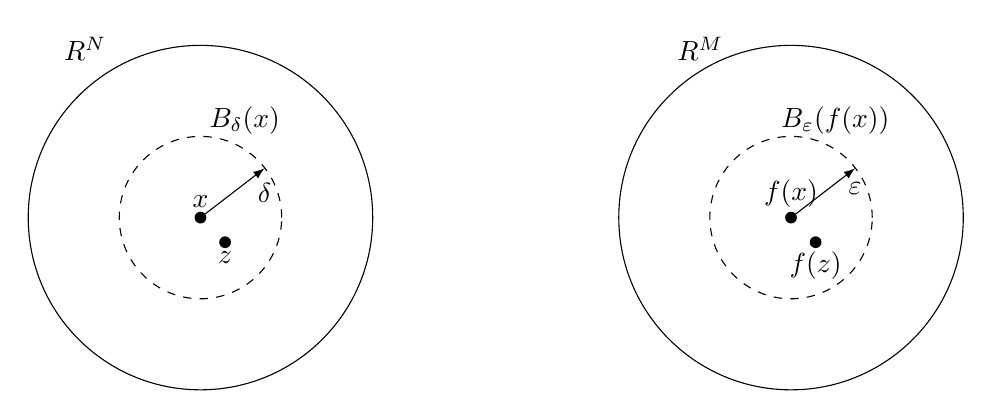
\begin{tikzpicture}[scale=1.25]
            % ------------------------------------------
            \node [above, align=flush center] at (-1.125, 1.5) {
                $\mathbb{R}^N$
            };
            \node at (0, 0) [circle, fill, inner sep = 1.5pt] {};
            \node[above] at (0, 0) {$x$};

            \node at (0.25, -0.25) [circle, fill, inner sep = 1.5pt] {};
            \node[below] at (0.25, -0.25) {$z$};

            \draw [dashed] (0, 0) circle [radius=0.825];
            \draw [-] (0, 0) circle [radius=1.750];

            \draw [->, >=latex] (0, 0) -- (0.65, 0.5)
              node[below] at (0.65, 0.45) {$\delta$};

            \node[above] at (0.45, 0.75) {$B_{\delta}(x)$};

            \node at (3, 0) {$\implies$};

            % ------------------------------------------
            \node [above, align=flush center] at (5.125, 1.5) {
                $\mathbb{R}^M$
            };
            \node at (6, 0) [circle, fill, inner sep = 1.5pt] {};
            \node[above] at (6, 0) {$f(x)$};

            \node at (6.25, -0.25) [circle, fill, inner sep = 1.5pt] {};
            \node[below] at (6.25, -0.25) {$f(z)$};

            \draw [->, >=latex] (6, 0) -- (6.65, 0.5)
              node[below] at (6.65, 0.45) {$\varepsilon$};

            \node[above] at (6.45, 0.75) {$B_{\varepsilon}(f(x))$};

            \draw [dashed] (6, 0) circle [radius=0.825];
            \draw [-] (6, 0) circle [radius=1.750];
          \end{tikzpicture}
        \end{figure}

        We want to show that if $O \subseteq \mathbb{R}^M$ is open, then $f^{-1}(O)$ is open. That is, $\forall x \in f^{-1}(O) ~~ \exists \delta > 0$ s.t. $z \in B_{\delta}(x) \implies z \in f^{-1}(O)$. You will note this is a very similar statement!
        \begin{figure}[H]
          \centering
          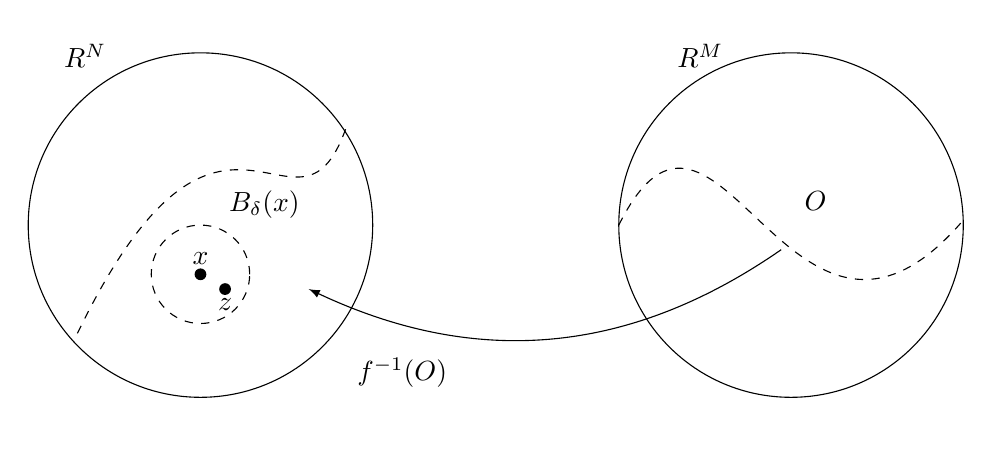
\begin{tikzpicture}[scale=1.25]
            % ------------------------------------------
            \node [above, align=flush center] at (-1.125, 1.5) {
                $\mathbb{R}^N$
            };
            \node at (0, -0.5) [circle, fill, inner sep = 1.5pt] {};
            \node[above] at (0, -0.5) {$x$};

            \node at (0.25, -0.65) [circle, fill, inner sep = 1.5pt] {};
            \node[below] at (0.25, -0.65) {$z$};

            \draw [dashed] (0, -0.5) circle [radius=0.5];
            \draw [-] (0, 0) circle [radius=1.750];
            \node[below] at (0.65, 0.45) {$B_{\delta}(x)$};

            \draw [dashed]
              (-1.25, -1.1)
                ..
                controls
                  (0.25, 2) and
                  (1, -0.5)
                ..
              (1.5, 1.05);

            % ------------------------------------------
            \node [above, align=flush center] at (5.125, 1.5) {
                $\mathbb{R}^M$
            };
            \draw [-] (6, 0) circle [radius=1.750];
            \draw [dashed]
              (4.25, 0)
                ..
                controls
                  (5.25, 2) and
                  (6, -2)
                ..
              (7.75, 0.05);
            \node[above] at (6.25, 0.05) {$O$};
            \draw [->, >=latex]
              (5.9, -0.25) to[bend left] (1.1, -0.65)
              node[below] at (2.05, -1.25) {$f^{-1}(O)$};
          \end{tikzpicture}
        \end{figure}

      \item It's basically the same picture: All we are missing is $B_{\varepsilon}(f(x))$ and it looks like we're done. How do we get it? We use the fact that $O$ is open in $\mathbb{R}^M$.
        \begin{figure}[H]
          \centering
          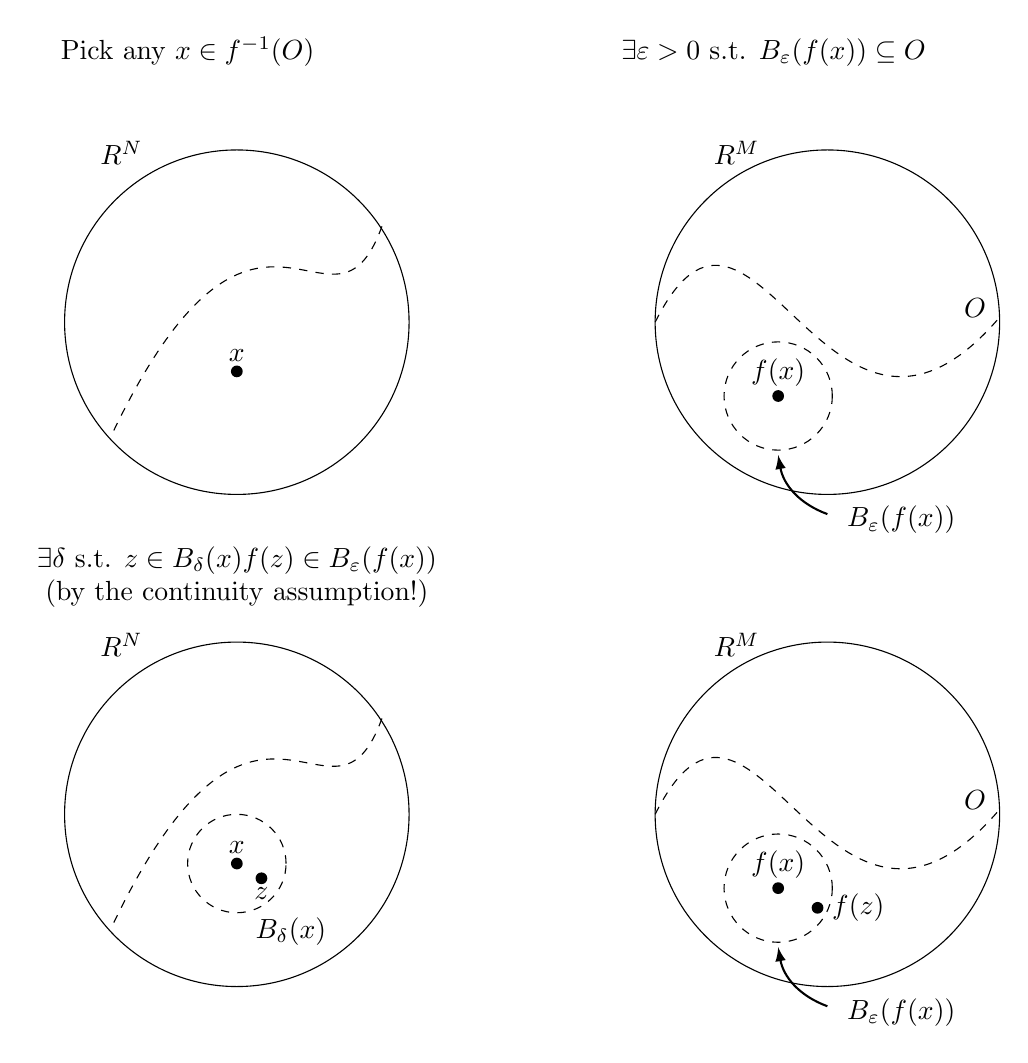
\begin{tikzpicture}[scale=1.25]
            % ------------------------------------------
            \node [above, align=flush center] at (-0.5, 2.5) {Pick any $x \in f^{-1}(O)$};
            \node [above, align=flush center] at (-1.125, 1.5) {
                $\mathbb{R}^N$
            };
            \node at (0, -0.5) [circle, fill, inner sep = 1.5pt] {};
            \node[above] at (0, -0.5) {$x$};

            \draw [-] (0, 0) circle [radius=1.750];
            \draw [dashed]
              (-1.25, -1.1)
                ..
                controls
                  (0.25, 2) and
                  (1, -0.5)
                ..
              (1.5, 1.05);

            % ------------------------------------------
            \node [above, align=flush center] at (5.5, 2.5) {
              $\exists \varepsilon > 0$ s.t. $B_{\varepsilon}(f(x)) \subseteq O$
            };
            \node [above, align=flush center] at (5.125, 1.5) {
                $\mathbb{R}^M$
            };
            \draw [-] (6, 0) circle [radius=1.750];
            \draw [dashed]
              (4.25, 0)
                ..
                controls
                  (5.25, 2) and
                  (6, -2)
                ..
              (7.75, 0.05);
            \node[above] at (7.5, -0.05) {$O$};

            \node[above] at (6.75, -2.25) {$B_{\varepsilon}(f(x))$};
            \draw [dashed] (5.5, -0.75) circle [radius=0.55];
            \draw [->, >=latex, line width=0.75pt] (6, -1.95) to[bend left] (5.5, -1.35) ;

            \node at (5.5, -0.75) [circle, fill, inner sep = 1.5pt] {};
            \node[above] at (5.5, -0.75) {$f(x)$};

            % ------------------------------------------
            \node [above, align=flush center] at (0, -3) {
              $\exists \delta$ s.t. $z \in B_{\delta}(x) \implies f(z) \in B_{\varepsilon}(f(x))$
              \\
              (by the continuity assumption!)
            };
            \node [above, align=flush center] at (-1.125, -3.5) {
                $\mathbb{R}^N$
            };
            \node at (0, -5.5) [circle, fill, inner sep = 1.5pt] {};
            \node[above] at (0, -5.5) {$x$};

            \node at (0.25, -5.65) [circle, fill, inner sep = 1.5pt] {};
            \node[below] at (0.25, -5.65) {$z$};

            \draw [dashed] (0, -5.5) circle [radius=0.5];
            \draw [-] (0, -5) circle [radius=1.750];
            \node[below] at (0.55, -5.95) {$B_{\delta}(x)$};

            \draw [dashed]
              (-1.25, -6.1)
                ..
                controls
                  (0.25, -3) and
                  (1, -5.5)
                ..
              (1.5, -3.95);

            % ------------------------------------------
            \node at (3, -5) {$\implies$};
            \node [above, align=flush center] at (5.125, -3.5) {
                $\mathbb{R}^M$
            };
            \draw [-] (6, -5) circle [radius=1.750];
            \draw [dashed]
              (4.25, -5)
                ..
                controls
                  (5.25, -3) and
                  (6, -7)
                ..
              (7.75, -4.95);
            \node[above] at (7.5, -5.05) {$O$};

            \node[above] at (6.75, -7.25) {$B_{\varepsilon}(f(x))$};
            \draw [dashed] (5.5, -5.75) circle [radius=0.55];
            \draw [->, >=latex, line width=0.75pt] (6, -6.95) to[bend left] (5.5, -6.35) ;

            \node at (5.5, -5.75) [circle, fill, inner sep = 1.5pt] {};
            \node[above] at (5.5, -5.75) {$f(x)$};

            \node at (5.9, -5.95) [circle, fill, inner sep = 1.5pt] {};
            \node[right] at (5.95, -5.95) {$f(z)$};
          \end{tikzpicture}
        \end{figure}

        Note $f(z) \in B_{\varepsilon}(f(x)) \subseteq O$, so $z \in f^{-1}(O)$. This statement is the heart of the proof! It is not obvious that $B_{\delta}(x)$ will be contained in $f^{-1}(O)$, so we need the link with $B_{\varepsilon}(f(x))$ we drew above. Only then can we say that for arbitrary $x$ we found $\delta > 0$ s.t. $z \in B_{\delta}(x) \implies z \in f^{-1}(O)$; by definition that means the set is open.
      \end{itemize}

    \item We show $c \iff b$. First, consider any closed set $S \in \mathbb{R}^M$, so $\mathbb{R}^M \setminus S$ is open; by premise, $f^{-1}(\mathbb{R}^M \setminus S)$ is also open, which means $\mathbb{R}^N \setminus f^{-1}(\mathbb{R}^M \setminus S) = f^{-1}(\mathbb{R}^N \setminus (\mathbb{R}^M \setminus S)) = f^{-1}(S)$ is closed. (The only sticking point here would be to show that in general $f^{-1}(\mathbb{R}^M \setminus O) = \mathbb{R}^N \setminus f^{-1}(O)$, which I trust you can do.\footnote{The way to prove two sets are equal is to show either set conains the other. Take any $x \in f^{-1}(\mathbb{R}^M \setminus O) \subseteq \mathbb{R}^N$, so $f(x) \in \mathbb{R}^M \setminus O$. If $x \in f^{-1}(O)$ then $f(x) \in O$, contradiction. Hence $x \in \mathbb{R}^N$ and $x \notin O$, so $x \in \mathbb{R}^N \setminus f^{-1}(O)$.  Pick $z \in \mathbb{R}^N \setminus f^{-1}(O)$. If $f(z) \in O$ then $z \in f^{-1}(O)$, contradiction. Hence $f(z) \in \mathbb{R}^M \setminus O$, which means $z \in f^{-1}(\mathbb{R}^M \setminus O)$.}) Now consider open set $O \in \mathbb{R}^M$, so $\mathbb{R}^M \setminus O$ is open; by premise, $f^{-1}(\mathbb{R}^M \setminus O)$ is also closed, which means $\mathbb{R}^N \setminus f^{-1}(\mathbb{R}^M \setminus O) = f^{-1}(O)$ is open. You will notice this is an entirely analogous argument.

      % xx you are here; check replacing with rr^n/m works

    \item For this one it is easier to show that $b \implies d$ (noting we already argued $c \implies b$).
      \begin{itemize}[label=$\bullet$]
        \item $\forall O \subseteq \mathbb{R}^M$, if $O$ open then $f^{-1}(O)$ open. This means that $\forall x \in f^{-1}(O)~~ \exists\delta$ s.t. $B_{\delta}(x) \subseteq f^{-1}(O)$.

        \item We WTS $x_m \to x \implies f(x_m) \to f(x)$; i.e.  $\forall \varepsilon > 0 ~~ \exists M$ s.t. $m \ge M \implies f(x_m) \in B_{\varepsilon}(f(x))$.

        % \item We are given the equivalent statement for $x_m$ and $x$; what we need to do is start in $\mathbb{R}^M$ and map back to $\mathbb{R}^N$, where we know we have a convergent sequence. This is where $f^{-1}(O)$ being open helps!
        \begin{figure}[H]
          \centering
          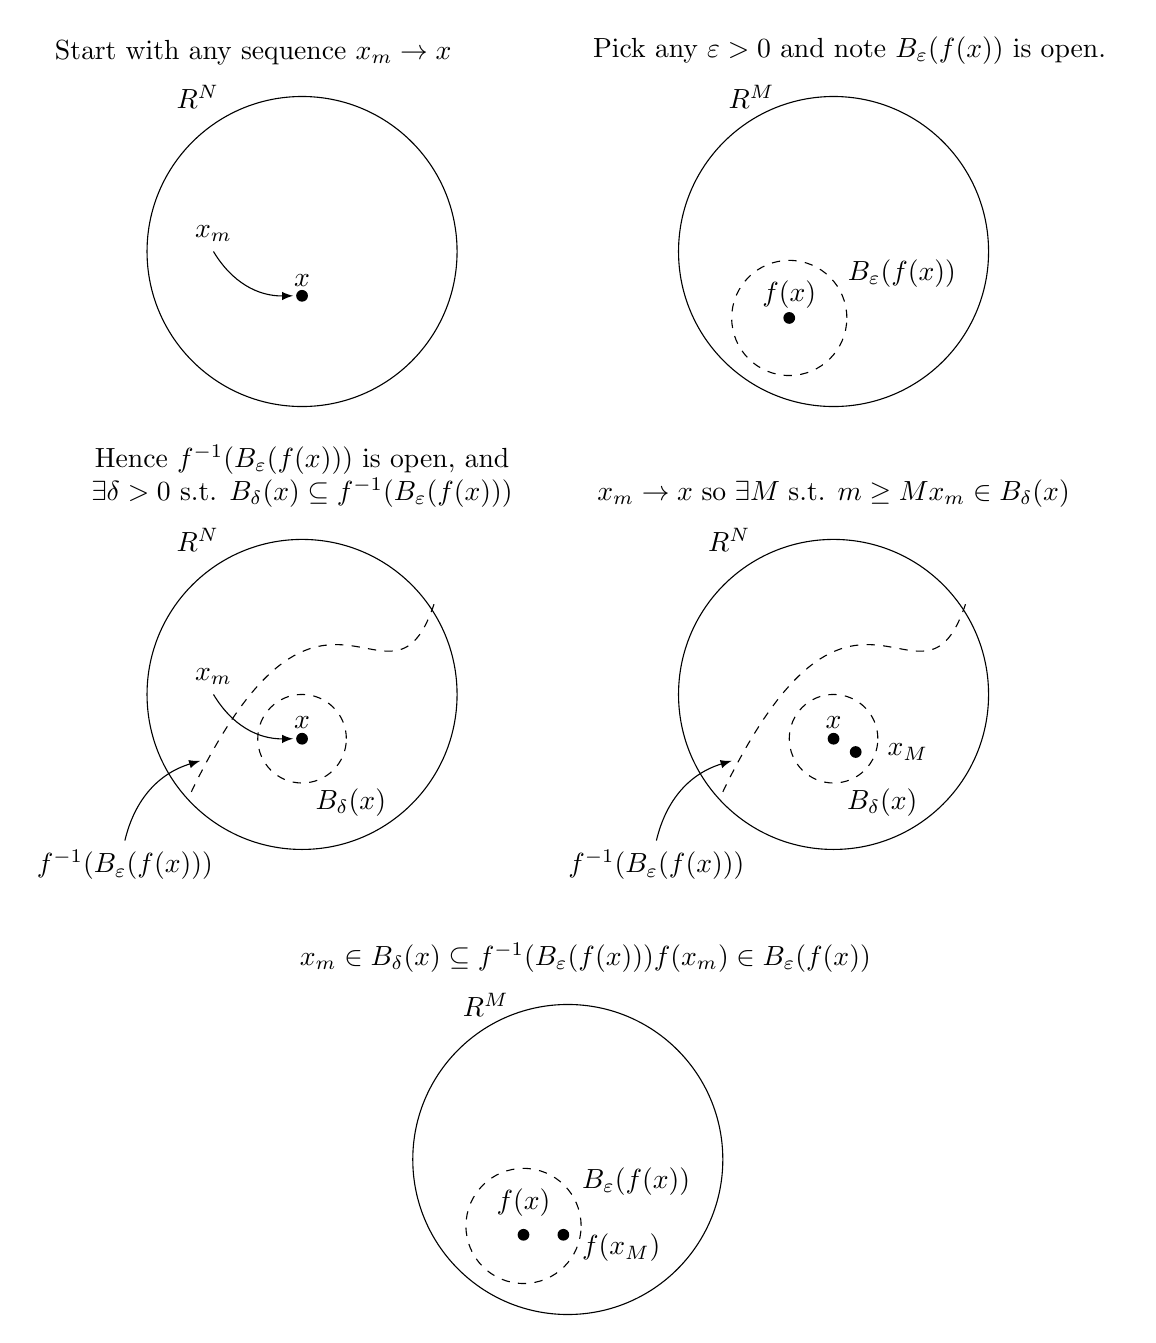
\begin{tikzpicture}[scale=1.125]
            % ------------------------------------------
            \node [above, align=flush center] at (-0.5, 2.5) {
              Start with any sequence $x_m \to x$
            };
            \node [above, align=flush center] at (-1.125, 2) {
                $\mathbb{R}^N$
            };
            \node at (0, 0) [circle, fill, inner sep = 1.5pt] {};
            \node[above] at (0, 0) {$x$};

            \draw [-] (0, 0.5) circle [radius=1.750];
            \draw [->, >=latex] (-1, 0.5) to[bend right] (-0.1, 0);
            \node[above] at (-1, 0.5) {$x_m$};

            % ------------------------------------------
            \node [above, align=flush center] at (6.25, 2.5) {
              Pick any $\varepsilon > 0$ and note  $B_{\varepsilon}(f(x))$ is open.
            };
            \node [above, align=flush center] at (5.125, 2) {
                $\mathbb{R}^M$
            };
            \draw [-] (6, 0.5) circle [radius=1.750];

            \draw [dashed] (5.5, -0.25) circle [radius=0.65];
            \node[right] at (6.05, 0.25) {$B_{\varepsilon}(f(x))$};

            \node at (5.5, -0.25) [circle, fill, inner sep = 1.5pt] {};
            \node[above] at (5.5, -0.25) {$f(x)$};

            % ------------------------------------------
            \node [above, align=flush center, text width = 6cm] at (0, -2.5) {
              Hence $f^{-1}(B_{\varepsilon}(f(x)))$ is open, and
              $\exists \delta > 0$ s.t. $B_{\delta}(x) \subseteq f^{-1}(B_{\varepsilon}(f(x)))$
            };
            \node [above, align=flush center] at (-1.125, -3) {
                $\mathbb{R}^N$
            };
            \node at (0, -5) [circle, fill, inner sep = 1.5pt] {};
            \node[above] at (0, -5) {$x$};

            \draw [dashed] (0, -5) circle [radius=0.5];
            \draw [-] (0, -4.5) circle [radius=1.750];
            \node[below] at (0.55, -5.45) {$B_{\delta}(x)$};

            \draw [->, >=latex] (-1, -4.5) to[bend right] (-0.1, -5);
            \node[above] at (-1, -4.5) {$x_m$};

            \draw [->, >=latex] (-2, -6.15) to[bend left] (-1.15, -5.25);
            \node[below] at (-2, -6.15) {$f^{-1}(B_{\varepsilon}(f(x)))$};

            \draw [dashed]
              (-1.25, -5.6)
                ..
                controls
                  (0.25, -2.5) and
                  (1, -5)
                ..
              (1.5, -3.45);

            % ------------------------------------------
            \node [above, align=flush center, text width = 6cm] at (6, -2.5) {
              $x_m \to x$ so $\exists M$ s.t. $m \ge M \implies x_m \in B_{\delta}(x)$
            };
            \node [above, align=flush center] at (4.875, -3) {
                $\mathbb{R}^N$
            };
            \node at (6, -5) [circle, fill, inner sep = 1.5pt] {};
            \node[above] at (6, -5) {$x$};

            \draw [dashed] (6, -5) circle [radius=0.5];
            \draw [-] (6, -4.5) circle [radius=1.750];
            \node[below] at (6.55, -5.45) {$B_{\delta}(x)$};

            \node at (6.25, -5.15) [circle, fill, inner sep = 1.5pt] {};
            \node[right] at (6.5, -5.15) {$x_M$};

            \draw [->, >=latex] (4, -6.15) to[bend left] (4.85, -5.25);
            \node[below] at (4, -6.15) {$f^{-1}(B_{\varepsilon}(f(x)))$};

            \draw [dashed]
              (4.75, -5.6)
                ..
                controls
                  (6.25, -2.5) and
                  (7, -5)
                ..
              (7.5, -3.45);

            % ------------------------------------------
            \node [above, align=flush center] at (3.25, -7.75) {
              $x_m \in B_{\delta}(x) \subseteq f^{-1}(B_{\varepsilon}(f(x))) \implies f(x_m) \in B_{\varepsilon}(f(x))$
            };
            \node [above, align=flush center] at (2.125, -8.25) {
                $\mathbb{R}^M$
            };
            \draw [-] (3, -9.75) circle [radius=1.750];

            \draw [dashed] (2.5, -10.5) circle [radius=0.65];
            \node[right] at (3.05, -10) {$B_{\varepsilon}(f(x))$};

            \node at (2.5, -10.6) [circle, fill, inner sep = 1.5pt] {};
            \node[above] at (2.5, -10.5) {$f(x)$};

            \node at (2.95, -10.6) [circle, fill, inner sep = 1.5pt] {};
            \node[right] at (3.05, -10.75) {$f(x_M)$};

          \end{tikzpicture}
        \end{figure}

        Hence for any $x_m \to x$, for any $\varepsilon > 0$ we found $M$ s.t.
        \begin{align*}
          m \ge M
          \implies
          x_m \in f^{-1}(B_{\varepsilon}(f(x)))
          \implies f(x_m) \in B_{\varepsilon}(f(x))
        \end{align*}

        which by definition means $f(x_m) \to f(x)$.  The tricky step here was that $f^{-1}(B_{\varepsilon}(f(x)))$ does not need to be a nice set. We need the premise that the inverse image of open sets is open so that we can fit a neighborhood inside of it, and \textit{then} use the fact $x_m \to x$.
      \end{itemize}

    \item Finally, we show that $d \implies a$. We do this by contradiction.
      \begin{itemize}[label=$\bullet$]
        \item It is not clear why contradiction is the way to go; it boils down to the fact I think it's easier, but I don't think that's obvious. In general, if unsure how to start a proof, one strategy is to try to make progress with a direct proof, and if you get stuck, switch to contradiction or contrapositive to see if it helps.

        \item First, we have $x_m \to x \implies f(x_m) \to f(x)$.
        \begin{figure}[H]
          \centering
          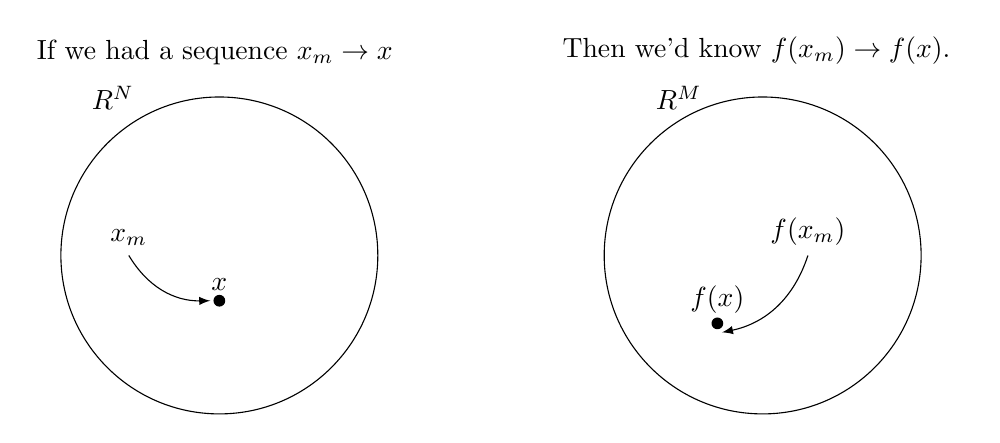
\begin{tikzpicture}[scale=1.15]
            % ------------------------------------------
            \node [above, align=flush center] at (0, 2.5) {
              If we had a sequence $x_m \to x$
            };
            \node [above, align=flush center] at (-1.125, 2) {
                $\mathbb{R}^N$
            };
            \node at (0, 0) [circle, fill, inner sep = 1.5pt] {};
            \node[above] at (0, 0) {$x$};

            \draw [-] (0, 0.5) circle [radius=1.750];
            \draw [->, >=latex] (-1, 0.5) to[bend right] (-0.1, 0);
            \node[above] at (-1, 0.5) {$x_m$};

            % ------------------------------------------
            \node at (3, 0) {$\implies$};

            \node [above, align=flush center] at (6, 2.5) {
              Then we'd know $f(x_m) \to f(x)$.
            };
            \node [above, align=flush center] at (5.125, 2) {
                $\mathbb{R}^M$
            };
            \draw [-] (6, 0.5) circle [radius=1.750];

            \node at (5.5, -0.25) [circle, fill, inner sep = 1.5pt] {};
            \node[above] at (5.5, -0.25) {$f(x)$};

            \draw [->, >=latex] (6.5, 0.5) to[bend left] (5.55, -0.35);
            \node[above] at (6.5, 0.5) {$f(x_m)$};
          \end{tikzpicture}
        \end{figure}

        \item We want to show that $\forall x \in \mathbb{R}^N ~~ \forall \varepsilon > 0 ~~ \exists \delta > 0$ s.t. $z \in B_{\delta}(x) \implies f(z) \in B_{\varepsilon}(f(x))$.

        \item A great starting point is to construct a sequence in $\mathbb{R}^N$ that converges to $x$, because the premise here is a statement about sequences. I don't see an obvious way to do this directly, but if we think about doing contradiction, we can negate the previous bullet point:
          \begin{align*}
            \exists x \in \mathbb{R}^N
            ~~
            \exists \varepsilon > 0
            ~~\text{s.t.}~~
            \forall \delta > 0
            ~~
            \exists z \in B_{\delta}(x)
            ~~\text{and}~~
            f(z) \notin B_{\varepsilon}(f(x))
          \end{align*}

          Note that $x$ and $\varepsilon$ here are fixed, and that we don't get to choose $z$---all we know is one such a $z$ exists. However, $\delta$ is a free parameter here, because this must be true for any $\delta$.

        \item If we pick $\delta = 1/m$ then we can construct a sequence $x_m \to x$ s.t. $f(x_m) \notin B_{\varepsilon}(f(x))$:
        \begin{figure}[H]
          \centering
          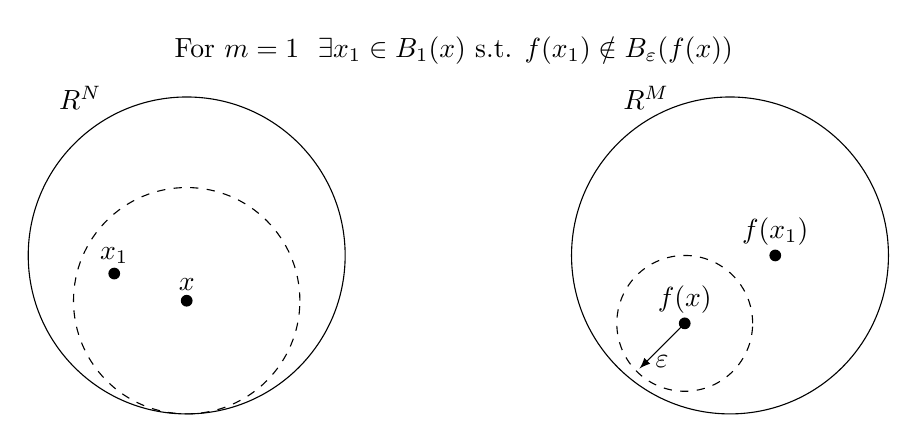
\begin{tikzpicture}[scale=1.15]
            \node [above, align=flush center] at (3, 2.5) {
                For $m = 1 ~~ \exists x_1 \in B_{1}(x)$ s.t. $f(x_1) \notin B_{\varepsilon}(f(x))$
              };

            % ------------------------------------------
            \node [above, align=flush center] at (-1.125, 2) {
                $\mathbb{R}^N$
            };
            \node at (0, 0) [circle, fill, inner sep = 1.5pt] {};
            \node[above] at (0, 0) {$x$};
            \draw [dashed] (0, 0) circle [radius=1.25];

            \draw [-] (0, 0.5) circle [radius=1.750];

            \node at (-0.8, 0.3) [circle, fill, inner sep = 1.5pt] {};
            \node[above] at (-0.8, 0.3) {$x_1$};

            % ------------------------------------------
            \node [above, align=flush center] at (5.125, 2) {
                $\mathbb{R}^M$
            };
            \draw [-] (6, 0.5) circle [radius=1.750];

            \node at (5.5, -0.25) [circle, fill, inner sep = 1.5pt] {};
            \node at (6.5, 0.5) [circle, fill, inner sep = 1.5pt] {};

            \draw [dashed] (5.5, -0.25) circle [radius=0.75];
            \draw [->, >=latex] (5.5, -0.25) -- (5, -0.75)
              node[below] at (5.25, -0.5) {$\varepsilon$};

            \node[above] at (5.5, -0.25) {$f(x)$};
            \node[above] at (6.5, 0.5) {$f(x_1)$};
          \end{tikzpicture}
        \end{figure}

        \begin{figure}[H]
          \centering
          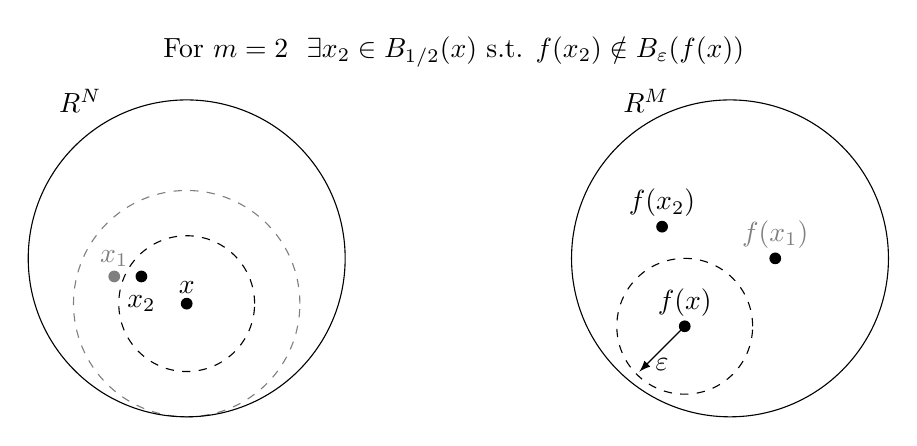
\begin{tikzpicture}[scale=1.15]
            \node [above, align=flush center] at (3, 2.5) {
                For $m = 2 ~~ \exists x_2 \in B_{1/2}(x)$ s.t. $f(x_2) \notin B_{\varepsilon}(f(x))$
              };

            % ------------------------------------------
            \node [above, align=flush center] at (-1.125, 2) {
                $\mathbb{R}^N$
            };
            \node at (0, 0) [circle, fill, inner sep = 1.5pt] {};
            \node[above] at (0, 0) {$x$};
            \draw [dashed, opacity = 0.5] (0, 0) circle [radius=1.25];
            \draw [dashed] (0, 0) circle [radius=0.75];

            \draw [-] (0, 0.5) circle [radius=1.750];

            \node at (-0.8, 0.3) [circle, fill, inner sep = 1.5pt, opacity = 0.5] {};
            \node[above, opacity = 0.5] at (-0.8, 0.3) {$x_1$};

            \node at (-0.5, 0.3) [circle, fill, inner sep = 1.5pt] {};
            \node[below] at (-0.5, 0.2) {$x_2$};

            % ------------------------------------------
            \node [above, align=flush center] at (5.125, 2) {
                $\mathbb{R}^M$
            };
            \draw [-] (6, 0.5) circle [radius=1.750];

            \node at (5.5, -0.25) [circle, fill, inner sep = 1.5pt] {};
            \node at (6.5, 0.5)   [circle, fill, inner sep = 1.5pt] {};
            \node at (5.25, 0.85) [circle, fill, inner sep = 1.5pt] {};

            \draw [dashed] (5.5, -0.25) circle [radius=0.75];
            \draw [->, >=latex] (5.5, -0.25) -- (5, -0.75)
              node[below] at (5.25, -0.5) {$\varepsilon$};

            \node[above] at (5.5, -0.25) {$f(x)$};
            \node[above, opacity=0.5] at (6.5, 0.5) {$f(x_1)$};
            \node[above] at (5.25, 0.85) {$f(x_2)$};
          \end{tikzpicture}
        \end{figure}

        \begin{figure}[H]
          \centering
          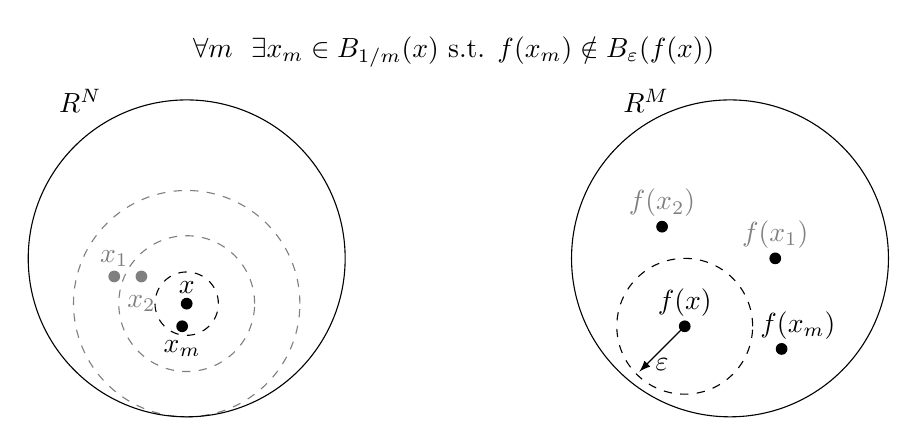
\begin{tikzpicture}[scale=1.15]
            \node [above, align=flush center] at (3, 2.5) {
                $\forall m ~~ \exists x_m \in B_{1/m}(x)$ s.t. $f(x_m) \notin B_{\varepsilon}(f(x))$
              };

            % ------------------------------------------
            \node [above, align=flush center] at (-1.125, 2) {
                $\mathbb{R}^N$
            };
            \node at (0, 0) [circle, fill, inner sep = 1.5pt] {};
            \node[above] at (0, 0) {$x$};
            \draw [dashed, opacity = 0.5] (0, 0) circle [radius=1.25];
            \draw [dashed, opacity = 0.5] (0, 0) circle [radius=0.75];
            \draw [dashed] (0, 0) circle [radius=0.35];

            \draw [-] (0, 0.5) circle [radius=1.750];

            \node at (-0.8, 0.3) [circle, fill, inner sep = 1.5pt, opacity = 0.5] {};
            \node[above, opacity = 0.5] at (-0.8, 0.3) {$x_1$};

            \node at (-0.5, 0.3) [circle, fill, inner sep = 1.5pt, opacity = 0.5] {};
            \node[below, opacity = 0.5] at (-0.5, 0.2) {$x_2$};

            \node at (-0.05, -0.25) [circle, fill, inner sep = 1.5pt] {};
            \node[below] at (-0.05, -0.3) {$x_m$};

            % ------------------------------------------
            \node [above, align=flush center] at (5.125, 2) {
                $\mathbb{R}^M$
            };
            \draw [-] (6, 0.5) circle [radius=1.750];

            \draw [dashed] (5.5, -0.25) circle [radius=0.75];
            \draw [->, >=latex] (5.5, -0.25) -- (5, -0.75)
              node[below] at (5.25, -0.5) {$\varepsilon$};

            \node at (5.5, -0.25) [circle, fill, inner sep = 1.5pt] {};
            \node at (6.5, 0.5)   [circle, fill, inner sep = 1.5pt] {};
            \node at (5.25, 0.85) [circle, fill, inner sep = 1.5pt] {};
            \node at (6.57, -0.5) [circle, fill, inner sep = 1.5pt] {};

            \node[above] at (5.5, -0.25) {$f(x)$};
            \node[above, opacity=0.5] at (6.5, 0.5) {$f(x_1)$};
            \node[above, opacity=0.5] at (5.25, 0.85) {$f(x_2)$};
            \node[above] at (6.75, -0.5) {$f(x_m)$};
          \end{tikzpicture}
        \end{figure}

        We can see as $x_m$ becomes increasingly closer to $x$, $f(x_m)$ is always at least $\varepsilon$ away from $f(x)$. In other words, we have constructed a sequence $x_m \to x$ were $f(x_m) \cancel\to f(x)$, contradiction. \qedhere
      \end{itemize}
  \end{enumerate}
\end{proof}

% ---------------------------------------------------------------------
\subsection{Intermediate Value Theorem (IVT)}
\label{sub:intermediate_value_theorem_ivt_}

\begin{theorem}[Intermediate Value Theorem (IVT)]
  If $f: [a, b] \to \mathbb{R}$ is continuous in $[a, b]$ then
  \[
    \forall L: f(a) < L < f(b) ~~ \exists c \in [a, b] \quad\text{s.t.}\quad f(c) = L
  \]
\end{theorem}

\begin{figure}[H]
  \centering
  \begin{tikzpicture}
    \begin{axis}[name=plot1
      ,title={Continuous}
      ,width=9cm
      ,height=6.5cm
      ,ymin=0
      ,ymax=6
      ,xmin=1
      ,xmax=6
      ,domain=1.5:6
      %,ylabel=$y$
      %,xlabel=$x$
    ]
    \addplot [smooth] {-(0.1 * (x - 4)^3 - 0.2 * x^2 + 0.2 * x + 0.5)};
    \addplot [only marks, mark=*, mark size=1.25pt] coordinates {(4, 1.9)};
    \node[right] at (axis cs:4.05, 1.85) {$L = f(c)$};
    \draw [-, dashed, line width=0.5pt]
      (axis cs:4, 0) -- (axis cs:4, 1.9) -- (axis cs:0, 1.9)
      node[above] at (axis cs:1.15, 1.95) {$L$}
      node[right] at (axis cs:4, 0.2) {$c$};
    \end{axis}

    \begin{axis}[name=plot2
      ,title={Not Continuous}
      ,at={($(plot1.east) + (0.5cm, 0)$)}
      ,anchor=west
      ,width=9cm
      ,height=6.5cm
      ,ymin=0
      ,ymax=6
      ,xmin=1
      ,xmax=6
      ,domain=1.5:6
      %,ylabel=$y$
      %,xlabel=$x$
    ]
    \addplot [smooth, domain=1.5:4] {-(0.1 * (x - 4)^3 - 0.2 * x^2 + 0.2 * x + 0.5)};
    \addplot [smooth, domain=4:6]   {-(0.1 * (x - 4)^3 - 0.2 * x^2 + 0.2 * x - 0.5)};
    \addplot [only marks, mark=*, mark size=1.25pt] coordinates {(4, 1.9)};
    \addplot [only marks, mark=*, mark size=1.5pt, color=white] coordinates {(4, 2.9)};
    \addplot [only marks, mark=o, mark size=1.5pt] coordinates {(4, 2.9)};
    \node[above] at (axis cs:1.15, 2.45) {$L$};
    \draw [-, dashed, line width=0.5pt] (axis cs:1, 2.4)  -- (axis cs:6, 2.4);
    \node[above] at (axis cs:5, 2.4) {$\cancel\exists c: f(c) = L$};
    \end{axis}
  \end{tikzpicture}
  \caption{Intermediate Value Theorem (IVT)}
  \label{fig:intermediate_value_theorem_ivt}
\end{figure}

\begin{proof}
  Take $A = \set{x \in [a, b]: f(x) \le L}$. $A$ is bounded so the $\sup$ exists; let $c = \sup A$. For $\varepsilon_m = 1/m$ take $x_m \in (c - \varepsilon_m, c] \cap A$, so $x_m \to c$ and $f(x_m) \to f(c)$ (by continuity). Since $A$ is closed and $x_m \in A$, $c \in A$ and $f(c) \le L$. If $f(c) = L$ we are done; if $f(c) < L$ then, by continuity, for $\varepsilon: f(c) - \varepsilon < f(c) + \varepsilon < L ~~ \exists \delta$ s.t.
  \[
    x: c - \delta < c < x < c + \delta
    \implies
    |f(x) - f(c)| < \varepsilon
    \implies
    f(x) < L
    \implies
    x \in A
  \]

  Note $x > c$, but by definition of the $\sup$, $x \le \sup A = c$ for any $x \in A$, contradiction. Hence it must be that no such $x$ exists, which can only happen if $c = b$ ($c \in A \implies c \le b$ and $c < b$ means such an $x$ can exist). But this is another contradiction, since $b = c \implies f(b) = f(c) < L$, and by premise $L < f(b)$. Hence it must be that $f(c) = L$. (\NB: There was a question in class about  whether we might need to consider the $\inf$ as well, but this is not the case, as we arrive at a contradiction using just the $\sup$.)
\end{proof}

% ---------------------------------------------------------------------
\subsection{Fun Remarks}
\label{sub:fun_remarks}

You can have a fun relaxing minute listening to Tom Lehrer's \href{https://www.youtube.com/watch?v=zxFCQplZgKI#t=2m35s}{\textit{There's a Delta for Every Epsilon} \ExternalLink}:
\begin{quote}
There's a delta for every epsilon, \\
It's a fact that you can always count upon. \\
There's a delta for every epsilon \\
And now and again, \\
There's also an N. \\

But one condition I must give: \\
The epsilon must be positive \\
A lonely life all the others live, \\
In no theorem \\
A delta for them. \\

How sad, how cruel, how tragic, \\
How pitiful, and other adjec- \\
Tives that I might mention. \\
The matter merits our attention. \\
If an epsilon is a hero, \\
Just because it is greater than zero, \\
It must be mighty discouragin' \\
To lie to the left of the origin. \\

This rank discrimination is not for us, \\
We must fight for an enlightened calculus, \\
Where epsilons all, both minus and plus, \\
Have deltas \\
To call their own.
\end{quote}

\clearpage
\printindex

% ---------------------------------------------------------------------
\end{document}
